\documentclass[11pt]{article}
\usepackage[top=0in, bottom=0.5in, left=1in, right=1in]{geometry}
\usepackage[T1]{fontenc}
\usepackage[polish]{babel}
\usepackage[utf8]{inputenc}
\usepackage{lmodern}
\selectlanguage{polish}
\usepackage{graphicx}
\begin{document}
\title{Laboratorium 2}
\author{Jan Seredyński}
\date{\today}
\maketitle

\section{Wstęp}
Zadaniem laboratorium było opracowanie listy, stosu oraz kolejki, które dysponują funkcjami pop(), push(x), size() do ich sterowania.

\section{Sposób wykonania}
Do wykonania zadania zastosowałem liste dwukierunkową z metodami, które pozwalają na dodawanie oraz pobieranie danych zarówno z początku jak i końca listy. Nastepnie na bazie listy dziedziczyły klasy stosu i kolejki, które w dwoich metodach pop i push korzystaja z odpowiednich metod listy.

Wykonanlem przykładowa kolejke FIFO. Każda zmiana rodzaju kolejki będzie prosta dzięki implementacji listy dwukierunkowej. Dlatego nie tworzylem różnych rodzai kolejek.

\section{Funkcje dodatkowe}
Lista jest dwukierunkowa, po której dziedziczą stos i kolejka.

\section{Schematy odpowiednich struktur}

Lista dwukierunkowa
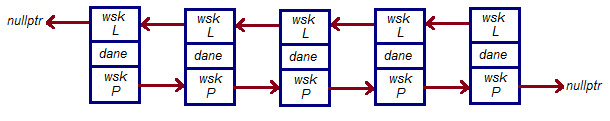
\includegraphics[width=5in]{lista2_1.png} 
\par\vspace{\baselineskip}
\hrule
\par\vspace{\baselineskip}
Stos, kolejka
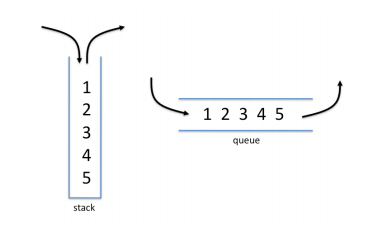
\includegraphics[width=3in]{stackqueue.png} 



\section{Podsumowanie}
Wszystkie zadania do laboratorium zostały wykonane poprawnie oraz zostały wprowadzone pewne dodatki jak np. lista dwukierunkowa.
\end{document}